%
% File iscol2018.tex

\documentclass[11pt,a4paper]{article}
\usepackage{natbib}
\usepackage{hyperref}
\usepackage{times}
\usepackage{latexsym}
\usepackage{amsmath}
\usepackage{tikz}
\usepackage{tikz-dependency}
\usepackage[warn]{textcomp}
\usepackage[font=small]{caption}
\usepackage{subcaption}
\usepackage{multirow}
\usepackage{url}
\usepackage{etoolbox}

\hyphenation{SemEval}

\DeclareMathOperator*{\argmin}{argmin}
\DeclareMathOperator*{\argmax}{argmax}

\makeatletter
\patchcmd\@combinedblfloats{\box\@outputbox}{\unvbox\@outputbox}{}{%
   \errmessage{\noexpand\@combinedblfloats could not be patched}%
}%
 \makeatother


\usetikzlibrary{shapes,shapes.misc}


\title{Multitask Parsing Across Semantic Representations}

\author{Daniel Hershcovich$^{1,2}$ \And
  Omri Abend$^2$ \And
  Ari Rappoport$^2$ \\
  $^1$The ESDPond and Lily Safra Center for Brain Sciences \\
  $^2$School of Computer Science and Engineering \\
  Hebrew University of Jerusalem \\
  \texttt{\{danielh,oabend,arir\}@cs.huji.ac.il}
}

\date{}

\begin{document}

\maketitle

Recent work in semantic parsing has targeted, among others,
Abstract Meaning Representation \cite[AMR;][]{banarescu2013abstract},
bilexical Semantic Dependencies \cite[SDP;][]{oepen2016towards}
and Universal Conceptual Cognitive Annotation \cite[UCCA;][]{abend2013universal}.
While these schemes are formally different and focus on different distinctions
(see Figure~\ref{fig:original_examples}),
much of their semantic content is shared \cite{abend2017state}.

We propose a general transition-based DAG parser,
able to parse UCCA, AMR, SDP and UD \cite{nivre2016universal}.
We train the parser using multitask learning (MTL)
to obtain significant improvements
on UCCA parsing over single-task training in
(1) in-domain and (2) out-of-domain settings in English;
(3) an in-domain setting in German; and
(4) an in-domain setting in French, where training data is
scarce.


\begin{figure}[!ht]
\fbox{\begin{subfigure}{0.47\textwidth}
  \centering
  \scalebox{.95}{
  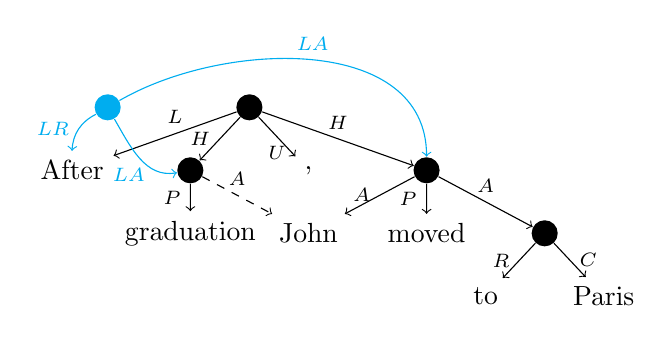
\begin{tikzpicture}[level distance=8mm, ->]
    \node (ROOT) [fill=black, circle] {}
      child {node (After) {After} edge from parent node[above] {\scriptsize $L$}}
      child {node (graduation) [fill=black, circle] {}
      {
        child {node {graduation} edge from parent node[left] {\scriptsize $P$}}
      } edge from parent node[left] {\scriptsize $H$} }
      child {node {,} edge from parent node[below] {\scriptsize $U$}}
      child {node (moved) [fill=black, circle] {}
      {
        child {node (John) {John} edge from parent node[left] {\scriptsize $A$}}
        child {node {moved} edge from parent node[left] {\scriptsize $P$}}
        child {node [fill=black, circle] {}
        {
          child {node {to} edge from parent node[left] {\scriptsize $R$}}
          child {node {Paris} edge from parent node[right] {\scriptsize $C$}}
        } edge from parent node[above] {\scriptsize $A$} }
      } edge from parent node[above] {\scriptsize $H$} }
      ;
    \draw[dashed,->] (graduation) to node [above] {\scriptsize $A$} (John);
    \node (LKG) at (-1.8,0) [fill=cyan, circle] {};
    \draw[bend right,color=cyan] (LKG) to node [auto, left] {\scriptsize $LR$} (After);
    \draw[color=cyan] (LKG) to[out=-60, in=190] node [below] {\scriptsize $LA\quad$} (graduation);
    \draw[color=cyan] (LKG) to[out=30, in=90] node [above] {\scriptsize $LA$} (moved);
  \end{tikzpicture}
  }\caption{UCCA \label{fig:original_example_ucca}}
\end{subfigure}}
\fbox{\begin{subfigure}{0.47\textwidth}
  \centering
  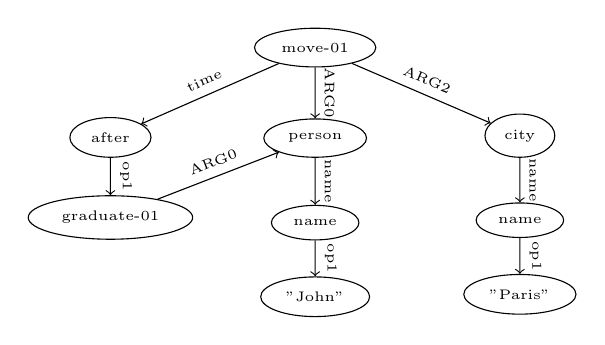
\begin{tikzpicture}[->,
      every node/.append style={sloped,anchor=south,auto=false,font=\tiny},
      level 1/.style={level distance=14mm,sibling distance=26mm},
      level 2/.style={level distance=13mm},
      level 3/.style={level distance=12mm}]
    \node (ROOT) [draw=black,ellipse] {move-01}
      child {node [draw=black,ellipse] {after}
      {
            child {node (graduation) [draw=black,ellipse] {graduate-01} edge from parent node {op1} }
      } edge from parent node {time} }
      child {node (John) [draw=black,ellipse] {person}
      {
        child {node [draw=black,ellipse] {name}
        {
            child {node [draw=black,ellipse] {"John"} edge from parent node {op1} }
        } edge from parent node {name} }
      } edge from parent node {ARG0} }
      child {node [draw=black,ellipse] {city}
      {
        child {node [draw=black,ellipse] {name}
        {
            child {node [draw=black,ellipse] {"Paris"} edge from parent node {op1} }
        } edge from parent node {name} }
      } edge from parent node {ARG2} }
      ;
      \draw (graduation) to node {ARG0} (John);
  \end{tikzpicture}
  \caption{AMR \label{fig:original_example_amr}}
\end{subfigure}}

\fbox{\begin{subfigure}{0.47\textwidth}
  \centering
    \begin{dependency}[text only label, label style={above}, font=\small]
    \begin{deptext}[column sep=.8em,ampersand replacement=\^]
    After \^ graduation \^ , \^ John \^ moved \^ to \^ Paris \\
    \end{deptext}
        \depedge[edge unit distance=1ex]{1}{2}{ARG2}
        \depedge[edge unit distance=1ex]{5}{4}{ARG1}
        \depedge[edge unit distance=1ex, edge end x offset=-2pt]{1}{5}{ARG1}
        \deproot[edge unit distance=1.5ex]{5}{top}
        \depedge[edge unit distance=2ex, edge start x offset=-1pt, edge end x offset=3pt]{5}{7}{ARG2}
        \depedge[edge unit distance=1ex, edge end x offset=5pt]{6}{5}{ARG1}
        \depedge[edge unit distance=1ex]{6}{7}{ARG2}
    \end{dependency}
  \caption{SDP \label{fig:original_example_sdp}}
\end{subfigure}}
\fbox{\begin{subfigure}{0.47\textwidth}
  \centering
    \begin{dependency}[text only label, label style={above}, font=\small]
    \begin{deptext}[column sep=.8em,ampersand replacement=\^]
    After \^ graduation \^ , \^ John \^ moved \^ to \^ Paris \\
    \end{deptext}
        \depedge[edge unit distance=1ex]{2}{1}{case}
        \depedge[edge unit distance=1ex]{4}{3}{punct}
        \depedge[edge unit distance=1ex]{5}{4}{nsubj}
        \depedge[edge unit distance=1ex, edge end x offset=-2pt]{2}{5}{obl}
        \depedge[edge unit distance=1ex]{7}{6}{case}
        \deproot[edge unit distance=1.5ex]{5}{root}
        \depedge[edge unit distance=1.5ex]{5}{7}{obl}
    \end{dependency}
  \caption{UD \label{fig:original_example_ud}}
\end{subfigure}}

\caption{\label{fig:original_examples}
 Example graph for each task.}
\end{figure}



%%%%%%%%%%%%%%%%%%%%%%%%%%%%%%%%%%%%%%%%%%%%%%%%%%%%%%%%%%%%%%%%%%%%%%%%%%%%%%%%%%%%%%%%%%%%
\paragraph{Multitask transition-based parsing.}

To parse graphs from all four tasks,
we extend TUPA \cite{hershcovich2017a}, 
a transition-based parser 
originally developed for UCCA.
TUPA's transition system can yield any labeled DAG
whose terminals are anchored in the text tokens.
We generalize TUPA so it can be applied to different tasks, 
and train it in a multitask setting.
The fairly small training set available for UCCA
makes MTL particularly appealing,
and we focus on it in this paper, treating AMR, SDP and UD parsing as auxiliary tasks.

\paragraph{Results.}
In an English in-domain setting, MTL with all auxiliary tasks and their combinations improves the primary $F_1$ score over
the single task baseline.
Using just SDP and UD as auxiliary tasks
yielded the best scores yet in in-domain UCCA parsing,
with 74.9\% $F_1$ on primary edges.

For English out-of-domain, improvements from using MTL are even more marked. 
The best model, using all three auxiliary tasks,
yields an error reduction of 2.9\%.
The contribution of MTL is also apparent in French and German in-domain parsing:
3.7\% error reduction in French
(having less than 10\% as much UCCA training data as English)
and 1\% in German, where the training set is comparable in size to the English one,
but is noisier.



\paragraph{Conclusion.}

We demonstrate that semantic parsers can leverage a range of 
semantically and syntactically annotated data, to improve their performance.
Our experiments show that MTL improves UCCA parsing,
using AMR, SDP and UD parsing as auxiliaries.



\bibliography{references}
\bibliographystyle{acl_natbib}

\end{document}
